% Se necesita un motor de LaTeX moderno como LuaLaTeX para compilar el documento
% debido al uso de fontspec y polyglossia
% Puede requerir tener el paquete lmodern instalado
% Se necesita ejecutar el compilador de LaTeX con -shell-escape
% Se necesita crear una carpeta llamada "tikz" en el directorio de compilación

% Declarar documento como tipo "article" a letra 12 puntos y tamaño de papel A4
\documentclass[12pt, a4paper]{article}

% Ampliar la superficie de papel usada por el documento
\usepackage[a4paper, total={6.5in, 9.5in}]{geometry}

% Configurar el idioma del documento a español
\usepackage{polyglossia}
\setdefaultlanguage{spanish}

% Generar marcadores de PDF a partir de los capítulos y secciones
\usepackage[bookmarks]{hyperref}

% Paquete para configuración avanzada de fuentes y uso de fuentes en formatos TTF y OTF
% Para que funcione es necesario usar un motor de LaTeX que lo soporte como LuaLaTeX
% https://en.wikibooks.org/wiki/LaTeX/Fonts#Using_TTF_and_OTF_fonts
\usepackage{fontspec}

% Paquete con herramientas para manejar colores en el documento
\usepackage[dvipsnames]{xcolor}

% Definiciones de color personalizadas
    % Comentarios en bloques de código (verde)
    \definecolor{code_comment}{rgb}{0, 0.5, 0}

% Paquete de herramientas matemáticas mejoradas
% https://en.wikibooks.org/wiki/LaTeX/Mathematics
% https://www.overleaf.com/learn/latex/Mathematical_expressions
% https://en.wikibooks.org/wiki/LaTeX/Advanced_Mathematics
\usepackage{mathtools}

% Símbolos matemáticos de la American Mathematical Society
% Entre estos símbolos se encuentran los que se usan para identificar conjuntos numéricos notables
% como el conjunto de los números enteros, números reales...
\usepackage{amssymb}

% Permite el posicionamiento preciso de figuras en la misma línea en la que se declaran
% https://www.overleaf.com/learn/latex/Positioning_images_and_tables#The_table_environment
\usepackage{float}

% Paquete que permite la creación de subfiguras dentro de un entorno de figura
% https://www.overleaf.com/learn/latex/Positioning_images_and_tables#Multiple_images_in_one_figure
\usepackage{subcaption}

% Paquete para poder declarar bloques de código con estilos
\usepackage{listings}

% Configuración general para los bloques de código
% https://en.wikibooks.org/wiki/LaTeX/Source_Code_Listings#Settings
\lstset{
    % Estilo del código
    basicstyle=\ttfamily,
    % Estilo de los comentarios
    commentstyle=\color{code_comment},
    % Habilitar numeración de líneas de código
    numbers=left,
    % Estilo de numeración de líneas de código
    numberstyle=\ttfamily,
    breaklines=true,
    language=Java
}

% Paquete para poder crear bordes alrededor del espacio que ocupa un entorno
\usepackage{framed}

% Paquete general para gráficos
% https://www.overleaf.com/learn/latex/TikZ_package
\usepackage{tikz}

% Paquete para crear diagramas
% https://www.overleaf.com/learn/latex/Pgfplots_package
\usepackage{pgfplots}

% Configurar versión de compatibilidad de pgfplots
% https://www.overleaf.com/learn/latex/Pgfplots_package#The_document_preamble
\pgfplotsset{compat=1.18}

% Habilitar generación de gráficas como archivos por separado
% Esto hace que el documento se compile más rápido ya que solo vuelve a generar
% las gráficas cuando estas son modificadas
% Para que el documento compile correctamente el motor de compilación se debe
% ejecutar con el argumento -shell-escape y se debe crear una carpeta llamada "tikz"
% en el directorio de compilación
\usetikzlibrary{external}
\usepgfplotslibrary{external}
\tikzexternalize[prefix=tikz/]

% Paquete para añadir imágenes
\usepackage{graphicx}
% Especificar directorio de imágenes
\graphicspath{ {./practica_8_memoria_resources/} }

% Paquete para bibliografías
% https://www.overleaf.com/learn/latex/Bibliography_management_with_biblatex
% https://en.wikibooks.org/wiki/LaTeX/Bibliography_Management
% https://en.wikibooks.org/wiki/LaTeX/Bibliography_Management#biblatex
\usepackage{biblatex}

% Añadir el archivo de referencias bibliográficas
\addbibresource{practica_8_memoria.bib}

% Definir un tipo de encabezado para bibliografías que permite generar una sección
% nueva con cada bibliografía que lo usa
\defbibheading{biblatex_encabezado_como_seccion}{\section{Bibliografía}}

\begin{document}
    % Portada personalizada
    % https://en.wikibooks.org/wiki/LaTeX/Title_Creation#Create_a_custom_title_for_a_report_or_book
    \begin{titlepage}
        % Centrar todo el contenido de la portada
        \centering
        
        % Nombre de la universidad en mayúsculas pequeñas (small caps)
        {\LARGE \textsc{Universidad Rey Juan Carlos} \par}

        % Nombre del grado
        {\Large Grado en Ingeniería de Computadores \par}

        % Curso
        {\large Curso 2023-2024 \par}

        % Espacio vertical
        \vspace{8cm}

        % Nombre de la asignatura
        {\Large \textsc{Fundamentos de diseño de software} \par}

        % Espacio vertical
        \vspace{0.5cm}
        
        % Número de la práctica
        {\huge Práctica 8: \par}

        % Nombre de la práctica en negrita
        {\Huge \bfseries Patrones de diseño de comportamiento \par}

        % Espacio vertical hasta abajo de la hoja
        \vfill

        % Autores
        {\LARGE Antonio Herman Boeriu \par}
        {\LARGE Yinghui Hu \par}
        {\LARGE Pablo Peral Camúñez \par}
    \end{titlepage}

    \section{Patrón iterador}

        \subsection{Diagrama UML}

            \begin{center}
                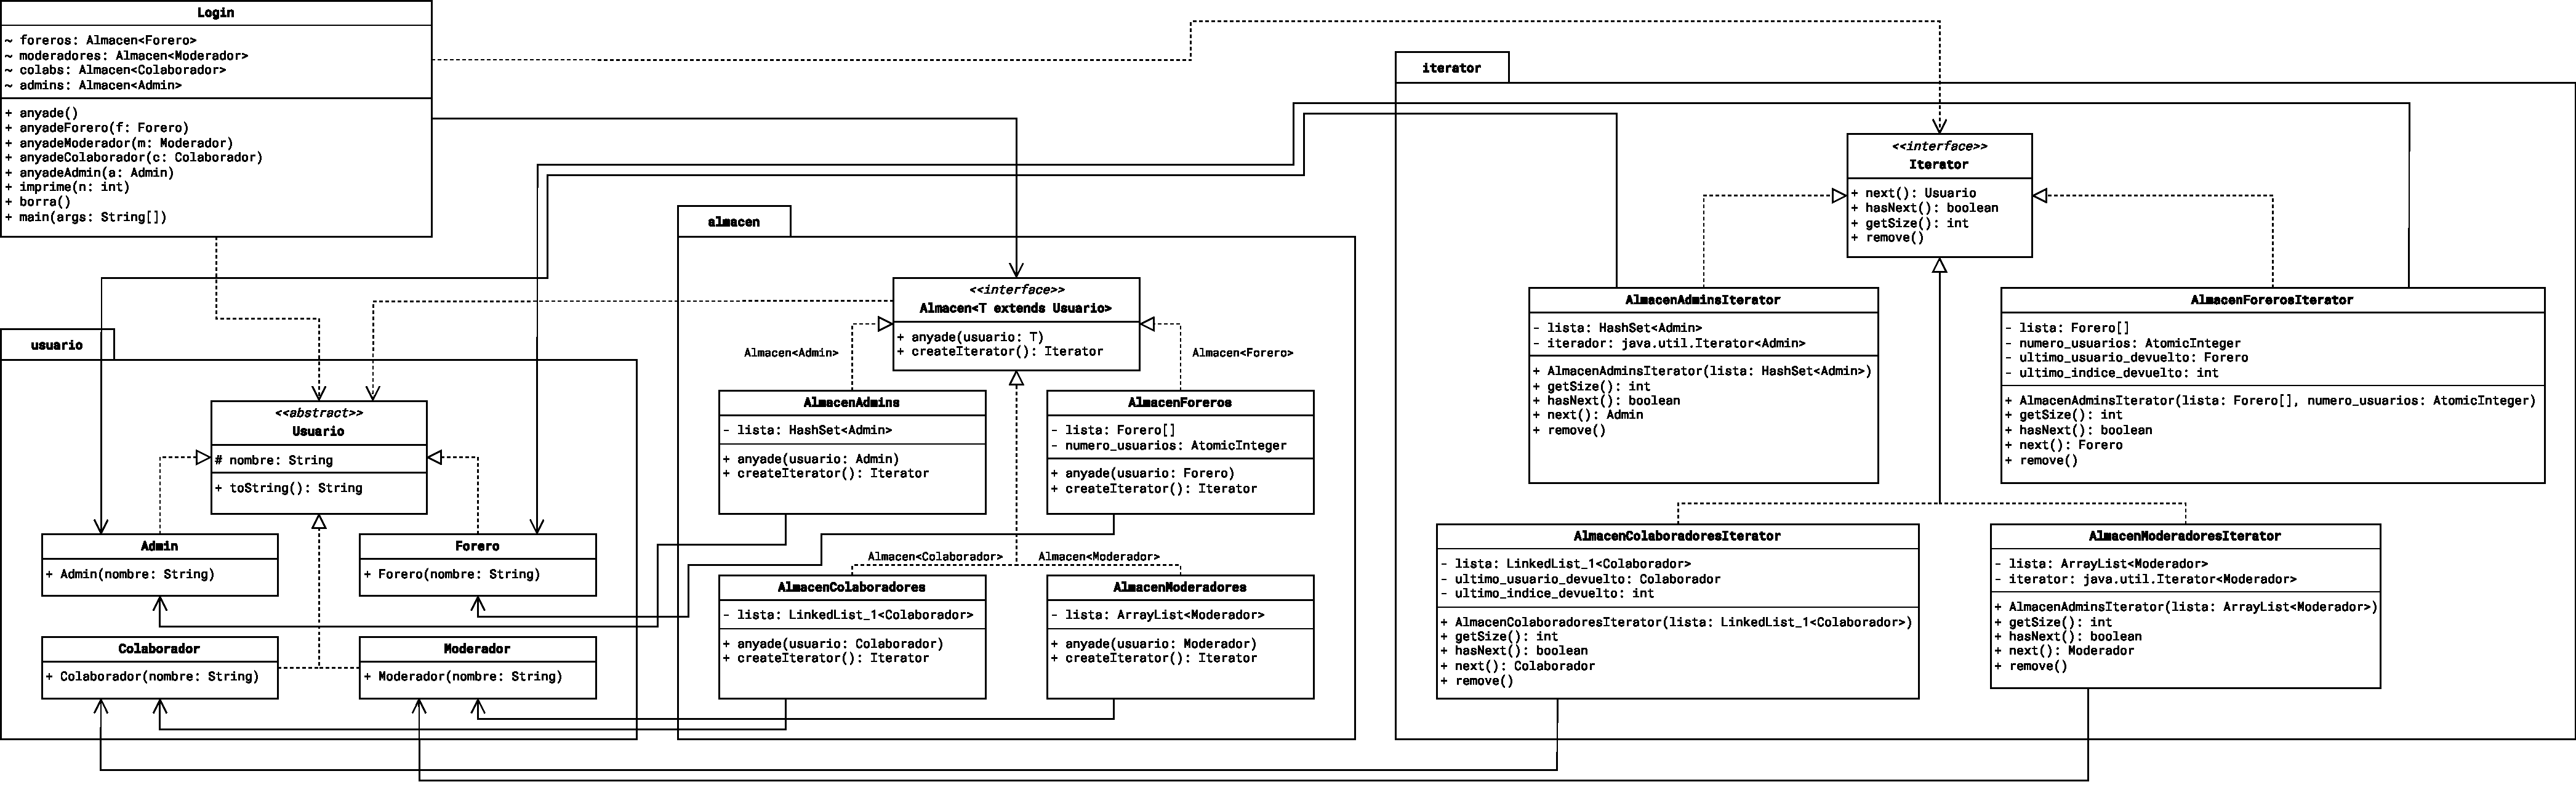
\includegraphics[width=\textwidth]{p8_ejercicio_1_uml.drawio.pdf}
            \end{center}

        \subsection{Código}

            \lstinputlisting[title=\lstname]{p8_ejercicio_1/src/main/java/com/example/usuario/Usuario.java}
            \lstinputlisting[title=\lstname]{p8_ejercicio_1/src/main/java/com/example/usuario/Admin.java}
            \lstinputlisting[title=\lstname]{p8_ejercicio_1/src/main/java/com/example/usuario/Colaborador.java}
            \lstinputlisting[title=\lstname]{p8_ejercicio_1/src/main/java/com/example/usuario/Forero.java}
            \lstinputlisting[title=\lstname]{p8_ejercicio_1/src/main/java/com/example/usuario/Moderador.java}            
            \lstinputlisting[title=\lstname]{p8_ejercicio_1/src/main/java/com/example/almacen/Almacen.java}
            \lstinputlisting[title=\lstname]{p8_ejercicio_1/src/main/java/com/example/almacen/AlmacenAdmins.java}
            \lstinputlisting[title=\lstname]{p8_ejercicio_1/src/main/java/com/example/almacen/AlmacenColaboradores.java}
            \lstinputlisting[title=\lstname]{p8_ejercicio_1/src/main/java/com/example/almacen/AlmacenForeros.java}
            \lstinputlisting[title=\lstname]{p8_ejercicio_1/src/main/java/com/example/almacen/AlmacenModeradores.java}
            \lstinputlisting[title=\lstname]{p8_ejercicio_1/src/main/java/com/example/iterator/Iterator.java}
            \lstinputlisting[title=\lstname]{p8_ejercicio_1/src/main/java/com/example/iterator/AlmacenAdminsIterator.java}
            \lstinputlisting[title=\lstname]{p8_ejercicio_1/src/main/java/com/example/iterator/AlmacenColaboradoresIterator.java}
            \lstinputlisting[title=\lstname]{p8_ejercicio_1/src/main/java/com/example/iterator/AlmacenForerosIterator.java}
            \lstinputlisting[title=\lstname]{p8_ejercicio_1/src/main/java/com/example/iterator/AlmacenModeradoresIterator.java}
            \lstinputlisting[title=\lstname]{p8_ejercicio_1/src/main/java/com/example/Login.java}


    \section{Patrón estrategia}

        \subsection{Diagrama UML}

            \begin{center}
                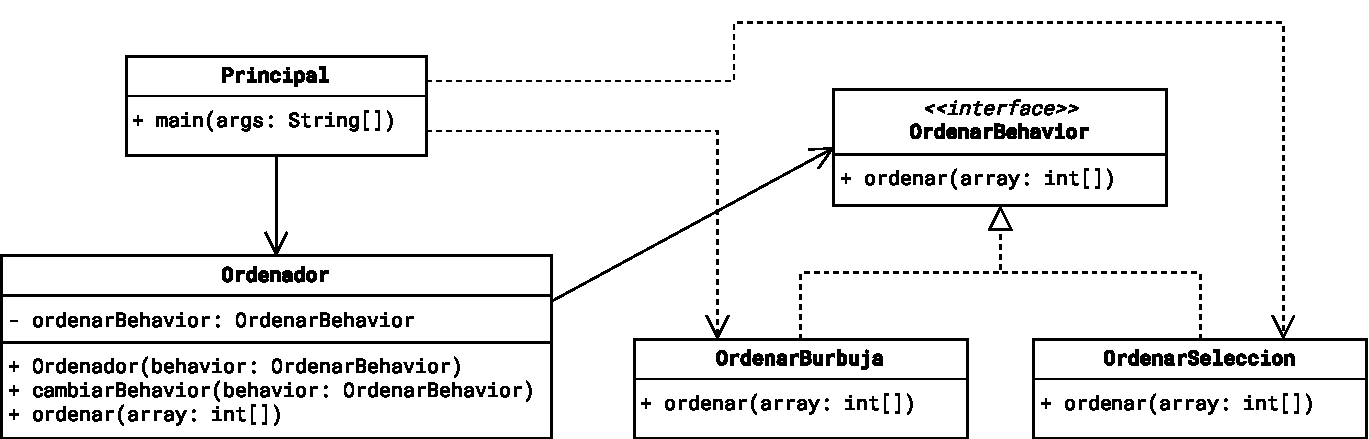
\includegraphics[width=\textwidth]{p8_ejercicio_2_uml.drawio.pdf}
            \end{center}
            
        \subsection{Código}

            \lstinputlisting[title=\lstname]{p8_ejercicio_2/src/main/java/com/example/Ordenador.java}
            \lstinputlisting[title=\lstname]{p8_ejercicio_2/src/main/java/com/example/OrdenarBehavior.java}
            \lstinputlisting[title=\lstname]{p8_ejercicio_2/src/main/java/com/example/OrdenarBurbuja.java}
            \lstinputlisting[title=\lstname]{p8_ejercicio_2/src/main/java/com/example/OrdenarSeleccion.java}
            \lstinputlisting[title=\lstname]{p8_ejercicio_2/src/main/java/com/example/Principal.java}

    \section{Patrón estado}

        \subsection{Diagrama UML}

            \begin{center}
                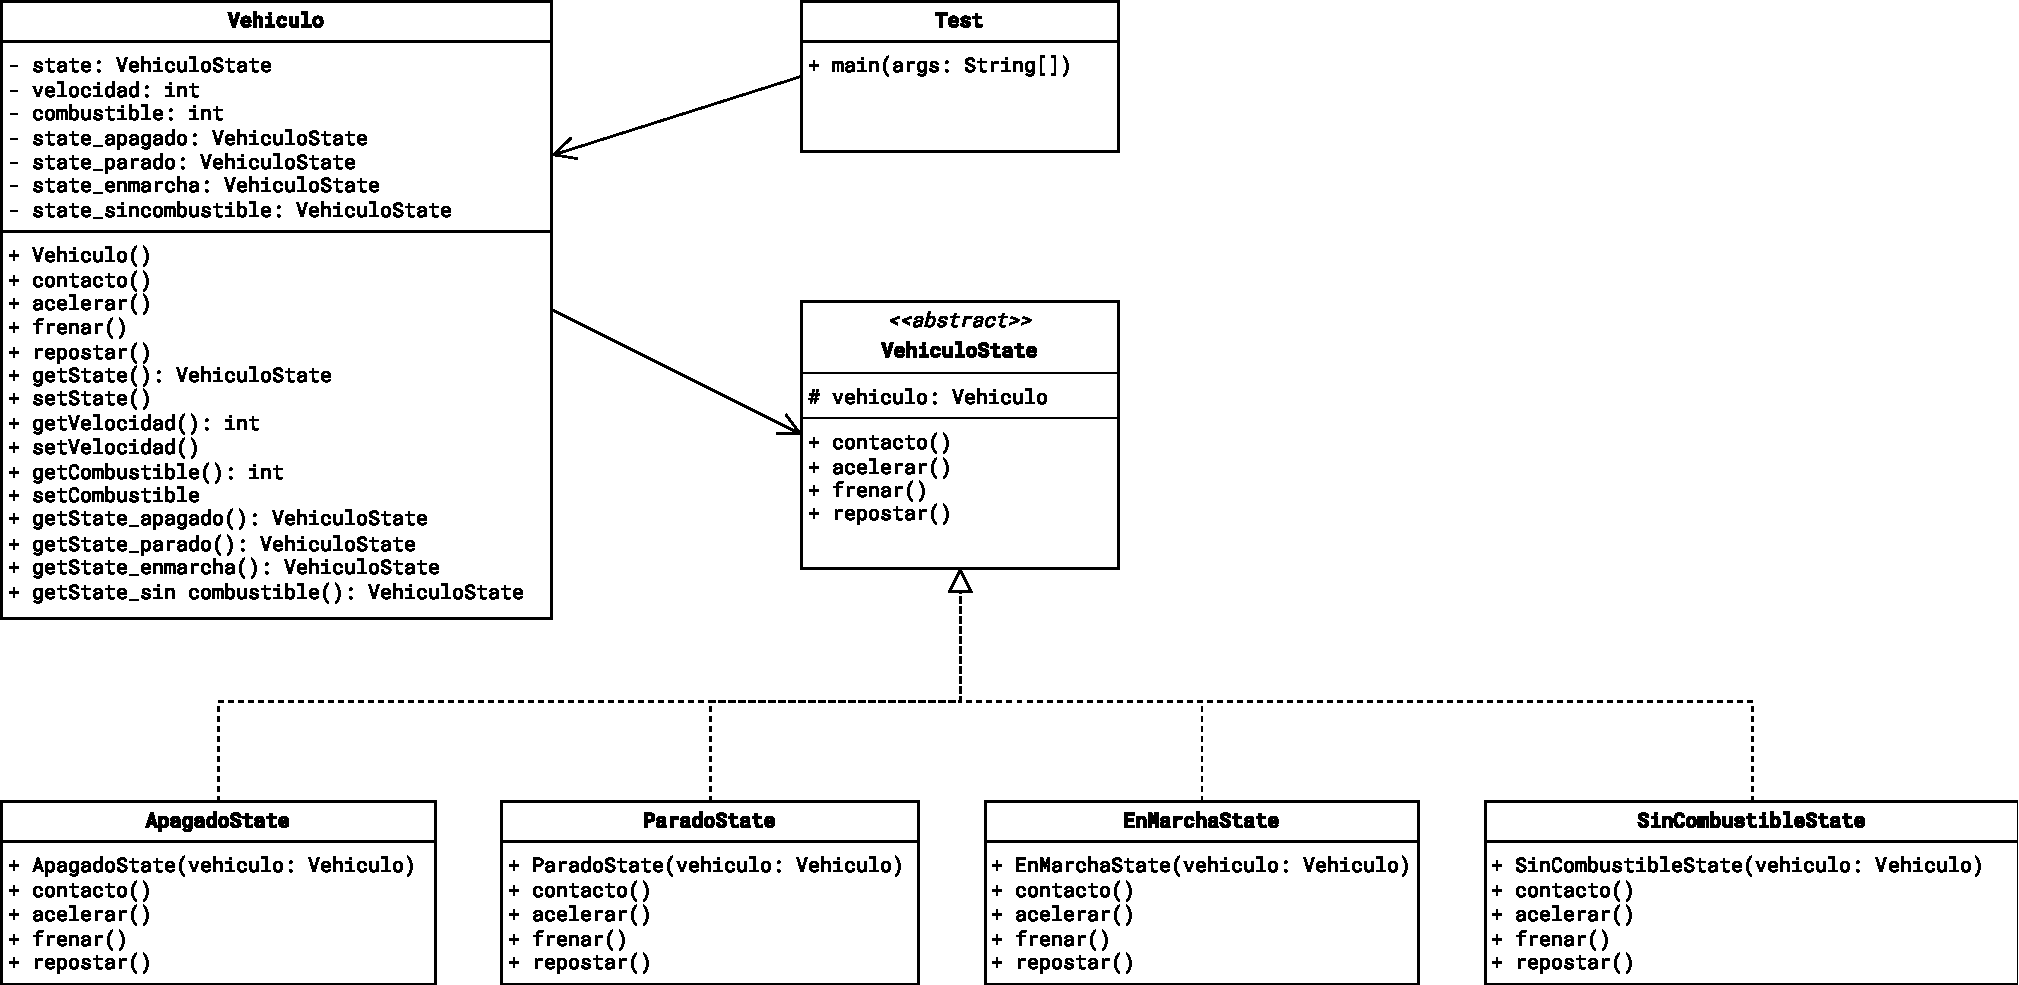
\includegraphics[width=\textwidth]{p8_ejercicio_3_uml.drawio.pdf}
            \end{center}

        \subsection{Código}

            \lstinputlisting[title=\lstname]{p8_ejercicio_3/src/main/java/com/example/VehiculoState.java}
            \lstinputlisting[title=\lstname]{p8_ejercicio_3/src/main/java/com/example/ApagadoState.java}
            \lstinputlisting[title=\lstname]{p8_ejercicio_3/src/main/java/com/example/ParadoState.java}
            \lstinputlisting[title=\lstname]{p8_ejercicio_3/src/main/java/com/example/EnMarchaState.java}
            \lstinputlisting[title=\lstname]{p8_ejercicio_3/src/main/java/com/example/SinCombustibleState.java}
            \lstinputlisting[title=\lstname]{p8_ejercicio_3/src/main/java/com/example/Vehiculo.java}
            \lstinputlisting[title=\lstname]{p8_ejercicio_3/src/main/java/com/example/Test.java}

\end{document}